\chapter{Opis projektnog zadatka}

\textit{Na osnovi projektnog zadatka detaljno opisati korisničke zahtjeve. Što jasnije opisati cilj projektnog zadatka, razraditi problematiku zadatka, dodati nove aspekte problema i potencijalnih rješenja. Očekuje se minimalno 3, a poželjno 4-5 stranica opisa.	Teme koje treba dodatno razraditi u ovom poglavlju su:}
		\begin{packed_item}
			\item \textit{potencijalna korist ovog projekta}
			\item \textit{postojeća slična rješenja (istražiti i ukratko opisati razlike u odnosu na zadani zadatak). Dodajte slike koja predočavaju slična rješenja.}
			\item \textit{skup korisnika koji bi mogao biti zainteresiran za ostvareno rješenje.}
			\item \textit{mogućnost prilagodbe rješenja }
			\item \textit{opseg projektnog zadatka}
			\item \textit{moguće nadogradnje projektnog zadatka}
		\end{packed_item}
		
		\textit{Za pomoć pogledati reference navedene u poglavlju „Popis literature“, a po potrebi konzultirati sadržaj na internetu koji nudi dobre smjernice u tom pogledu.}\vspace{0.5cm}
		
		{Porastom broja neprofitnih organizacija iz godine u godinu, raste i potreba za kvalitetnim aplikacijama koje bi takvim organizacijama omogućile nesmetan rad i funkcioniranje. Kako takve organizacije nisu u mogućnosti samostalno postići zadovoljavajuću razinu prihoda, to im postaje najveći problem te primorane su na suradnju s kompanijama sponzorima.}

		{Odaziv sponzora je često vrlo malen te je stoga potrebno kontaktirati velik broj kompanija. Praćenje statusa suradnji (uspješne / neuspješne) i osoba zaduženih za kontaktiranje sponzora vrlo brzo postaje kompleksno i neefikasno, a također dolazi i do mogućnosti curenja informacija. Raste potreba za aplikacijom koja će omogućiti evidenciju navedenih stavki te korisnicima dodijeliti razinu ovlasti kako bi umanjili mogućnost curenja informacija.}

		{Cilj ovog projekta je razviti programsku podršku za stvaranje web aplikacije \textit{”Company Database“} koja će služiti za evidenciju statusa suradnje kompanija na projektima i jednostavan uvid od strane \underbar{ovlaštenih} korisnika.}\vspace{0.2cm}
		

		{Korisnici će se u web aplikaciju prijavljivati koristeći Google račun koji mora biti registriran od strane drugih korisnika putem web aplikacije. Svaki je korisnik definiran sljedećim parametrima:}
		\begin{packed_item}
			\item {ime}
			\item {prezime}
			\item {korisnično ime} (nadimak)
			\item {opis}
			\item {email za login u aplikaciju}
			\item {email za obavijesti}
			\item {najviša razina ovlasti koju posjeduje (ukoliko je pripadnik više različitih razina ovlasti)}
		\end{packed_item}
		
		{Razlikovati ćemo 5 razina ovlasti, a to su redom od najviše prema najnižoj:}
		\begin{packed_item}
			\item {Administrator}
			\item {Moderator}
			\item {Fundraising (FR) responsible}
			\item {Fundraising (FR) team member}
			\item {Observer}
		\end{packed_item}

		{Svaki korisnik određene razine ovlasti ima sve mogućnosti svoje i svih nižih razina ovlasti sustava. Također ima mogućnost (kroz određene akcije) dodjeljivanja i oduzimanja \underbar{razina ovlasti} korisnicima nižih razina od svoje.}

		{Iznimke su administrator koji može dodijeliti i oduzeti i ostalim administratorima sustava te FR team member koji ne može dodijeliti niti oduzeti ovlasti jer se observer automatski dodjeljuje svim korisnicima koja nemaju višu razinu ovlasti.}\vspace{0.3cm}
		
		
		{\underbar{Administrator} može dodati, izmijeniti i obrisati korisnika.}\vspace{0.1cm}

		{\underbar{Moderator} može dodati i obrisati kategoriju projekata, stvoriti, izmijeniti i obrisati vlastito stvorene projekte. Pri stvaranju i izmjeni projekta, moderator mora odabrati korisnika koji će biti FR responsible za taj projekt te se tada tom korisniku dodijeljuje razina ovlasti FR responsible za taj projekt.}\vspace{0.1cm}

		{\underbar{FR responsible} može za dodijeljeni projekt dodati korisnike pod FR team members te stvoriti, modificirati i izbrisati suradnju s kompanijom iz popisa kompanija. Za svaku suradnju potrebno je odabrati odgovornog korisnika iz popisa FR team members koji u tom trenutku dobiva na email obavijest o zaduženju. Također može stvoriti, modificirati i obrisati vlastito stvorene kompanije.}\vspace{0.1cm}

		{\underbar{FR team member} ima mogućnost modifikacije statusa, kategorije, komentara i vrijednosti suradnje te pregleda svih podataka i izmjenu kontakata za dodjeljenu kompaniju. Također dobivaju obavijest („ping”) na email na datum prvog i drugog „pinga“ dodjeljenog projekta.}\vspace{0.1cm}

		{\underbar{Observer} ima mogućnost pregleda popisa svih korisnika, popisa svih projekata i popisa svih kompanija (naziv, područje, ABC kategorizacija, web URL) te pregleda informacija o projektu (naziv, kategorija, tip, datum početka, datum završetka, FR responsible)}\vspace{0.3cm}
		

		{\underbar{Projekt} je obilježen nazivom, kategorijom, tipom (interni ili eksterni), datumom početka i kraja, FR responsible-om zaduženim za navedeni projekt, popisom FR team member-a, FR ciljem (željeni prihod od projekta), prvim i drugom „pingom“ (timestamp) te popisom kompanija s kojima se surađuje na tom projektu.}\vspace{0.1cm}

		{\underbar{Kompanija} je obilježena nazivom, područjem kojim se bavi (npr. IT), ABC kategorizacijom, mjesecom planiranja budžeta, državom, poštanskim brojem, gradom, adresom, linkom na web stranicu, kratkim opisom, boolean varijablom \textit{„kontaktirati“} (koja označava treba li tu tvrtku u budućnosti kontaktirati) te popisom zaposlenika.}\vspace{0.1cm}
		
		{\underbar{Popis kompanija} moguće je uzlazno i silazno sortirati prema nazivu, području, mjesecu planiranja budžeta i linku na web stranicu te pretraživati po nazivu.}\vspace{0.1cm}

		{\underbar{Zaposlenik} kao entitet pripada kompaniji, a definiran je imenom, prezimenom, email adresom, brojem mobitela, ulogom u kompaniji (npr. CEO) te kratkim opisom.}\vspace{0.1cm}

		{\underbar{Suradnja} predstavlja poveznicu između projekta i kompanije, a obilježena je odgovornom osobom (koja je za nju zadužena), kontaktiranom osobom u kompaniji, kategorijom (financijska, materijalna ili akademska suradnja), vlastitim statusom (kontaktirano, ping, dopis, sastanak, uspješno ili neuspješno), komentarom (tj. sažetkom suradnje) te vrijednošću suradnje (koje se sumiraju i popunjavaju FR cilj projekta).}\vspace{0.3cm}

		{Aplikacija, sa svim navedenim funkcionalnostima i specifičnostima, biti će izvedena kao web aplikacija kojoj korisnici pristupaju pomoću Google autentifikatora. Biti će jednostavna za korištenje zahvaljujući preglednom i intuitivnom sučelju. Sustav će podržavati rad više korisnika u stvarnom vremenu, frontend će biti ostvaren u React-u, a backend će koristiti relacijsku bazu podataka i Spring boot.}

		\eject

\iffalse % block comment (zavrsava sa fi)

		\section{Primjeri u \LaTeX u}
		
		\textit{Ovo potpoglavlje izbrisati.}\\

		U nastavku se nalaze različiti primjeri kako koristiti osnovne funkcionalnosti \LaTeX a koje su potrebne za izradu dokumentacije. Za dodatnu pomoć obratiti se asistentu na projektu ili potražiti upute na sljedećim web sjedištima:
		\begin{itemize}
			\item Upute za izradu diplomskog rada u \LaTeX u - \url{https://www.fer.unizg.hr/_download/repository/LaTeX-upute.pdf}
			\item \LaTeX\ projekt - \url{https://www.latex-project.org/help/}
			\item StackExchange za Tex - \url{https://tex.stackexchange.com/}\\
		
		\end{itemize} 	

		%unos slike
		\begin{figure}[H]
			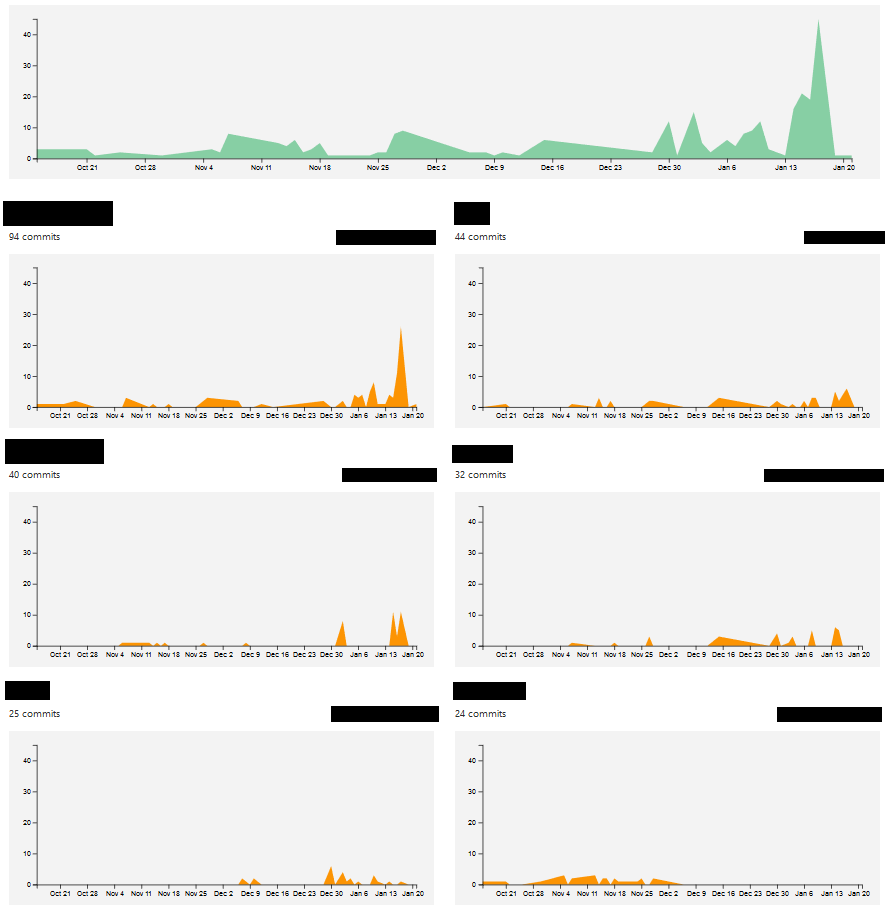
\includegraphics[scale=0.4]{slike/aktivnost.PNG} %veličina slike u odnosu na originalnu datoteku i pozicija slike
			\centering
			\caption{Primjer slike s potpisom}
			\label{fig:promjene}
		\end{figure}
		
		\begin{figure}[H]
			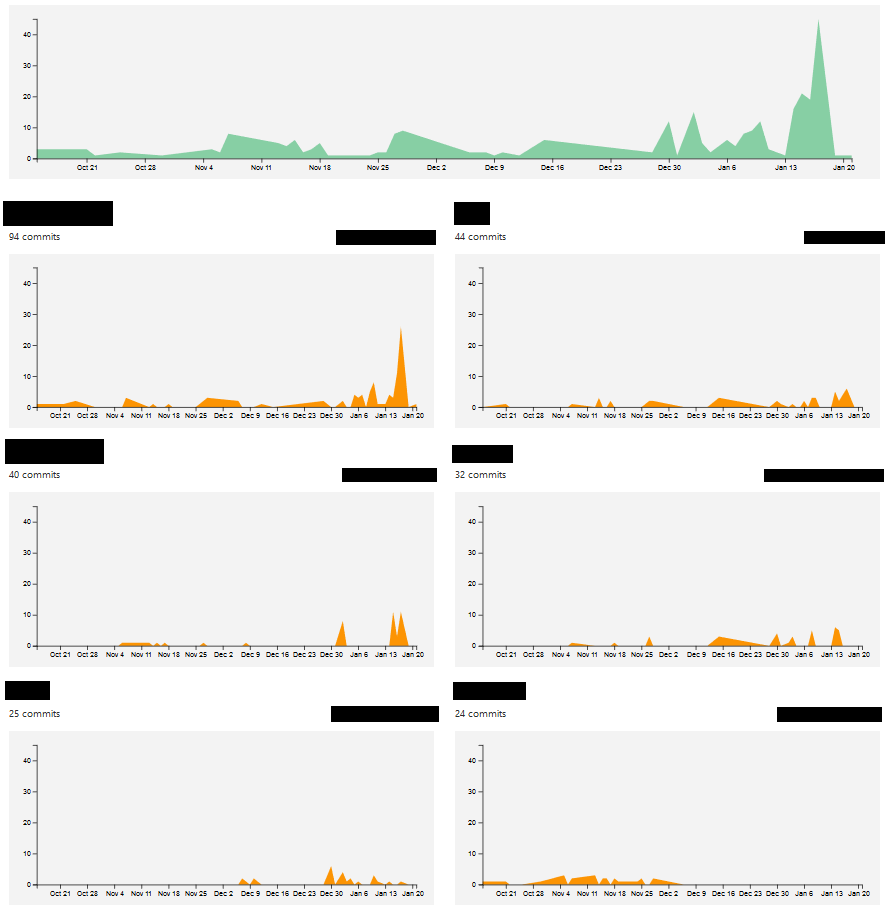
\includegraphics[width=\textwidth]{slike/aktivnost.PNG} %veličina u odnosu na širinu linije
			\caption{Primjer slike s potpisom 2}
			\label{fig:promjene2} %label mora biti drugaciji za svaku sliku
		\end{figure}
		
		Referenciranje slike \ref{fig:promjene2} u tekstu.
		\eject
		
\fi % block comment (pocinje sa iffalse)